\section{Theorie}
\label{sec:Theorie}
Nach dem Bohrschen Atommodell bewegen sich die Elektronen auf Schalen in diskreten Energiezuständen.
Die Elektronen können dabei unter Energiezufur auf eine höhere Schale wechseln.
Dieser Zustand $E_1$ ist allerdings nicht stabil, weshalb die Elektronen nach einer gewissen Zeit wieder in den Grundzustand $E_0$ zurückfallen.
Die zuvor aufgenommene Energie geben sie dabei in Form von Photonen einer gewissen Wellenlänge $\lambda$ ab.
Eine Möglichkeit Atomen beziehungsweise den entsprechenden Elektronen die nötige Energie zuzuführen, die sie brauchen um ihr Schale zu wechseln, ist sie mit Elektronen einer gewissen Energie zu beschießen.
Durch die Stöße können die Elektronen genug Energie zugeführt bekommen um ihren Energiezustand zu erhöhen.
Das Elektronen welches dabei für den Stoß genutzt wurde, verliert dabei den Teil der Energie, den das andere Elektron aufgenommen hat.
Für das freie Elektron bedeutet das, dies nun eine kleine kinetische Energie hat.
Die genaue Energie kann durch 
\begin{equation*}
    \frac{m_\text{e} v_0^2}{2} - \frac{m_\text{e}v_\text{after}^2}{2} = E_1 - E_0
\end{equation*} 
berechnet werden. $m_\text{e}$ entspricht dabei der Ruhemasse eines Elektrons, $v_0$ der Geschwindigkiet vor dem Stoß und $v_\text{after}$ der Geschwindigkeit des Elektrons nach dem Stoß.
\\\\
Der schematische Aufbau des Franck-Hertz Versuchs ist in Abbildung \ref{fig:schematischeraufbau} zu sehen.
\begin{figure}
    \centering
    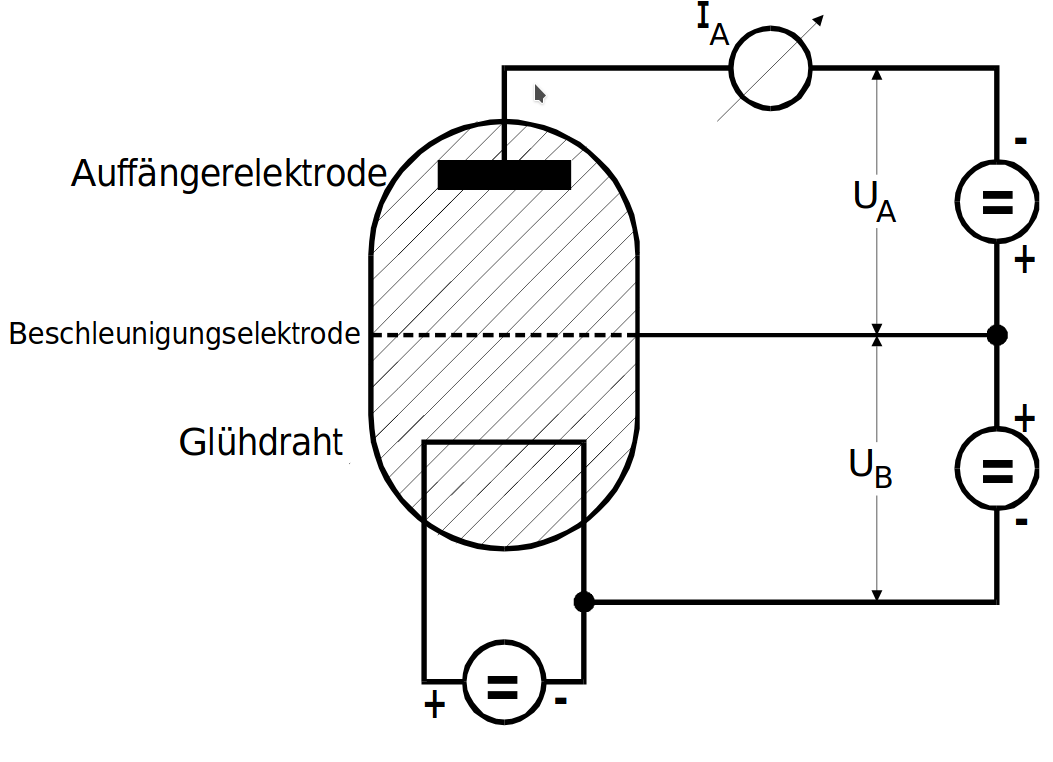
\includegraphics[width=0.75\textwidth]{content/data/schematischeraufbau.png}
    \caption{Der schematische Aufbau zum Franck-Hertz Versuch. Bild entnommen aus der Versuchsanleitung \cite[2]{anleitung}.}
    \label{fig:schematischeraufbau}
\end{figure}
Dieser besteht aus einer vakuumisierten Röhre, im linken Teil des Bildes, in welche ein Tropfen Quecksilber gegeben wird, welcher anschleißend verdampft.
In der Röhre befinden sich zudem ein Glühdraht, zur Erzeugung von Elektronen, eine Beschleunigungselektrode um die erzeugten Elektronen zu beschleunigen und eine Auffängerelektrode um zu messen wie viele Elektronen am Ende des Rohrs ankommen.
Es besteht die Möglichekit sowohl zwischen Glühdraht und Beschleunigungselektrode eine Spannung $U_\text{B}$ anzulegen als auch zwischen Beschelunigungselektrode und Auffängerelektrode $U_\text{A}$.
Durch die angelegte Spannung kann ein elektrisches Feld erzeugt werden, welches die Elektronen entweder bremst oder beschleunigt.
Die genau kinetische Energie nach durchlaufen der Beschleunigungsstrecke entspricht dabei, für Elektronen, dessen Startgeschwindigkeit 0 war
\begin{equation}
    \frac{m_\text{e} v^2}{2} = eU_\text{B},
    \label{eq:Energieelek}
\end{equation}
wobei $U_\text{B}$ der angelegten Spannung und $e$ der Elementarladung entspricht.
$v_\text{z}$ ist die Geschwindigkeit des Elektrons in z-Richtung, diese muss nach der Beschleunigung groß genug sein um das Gegenfeld zwischen Beschleunigungselektrode und Auffängerelektrode zu überwinden.
Es erreichen also nur Elektronen die Auffängerelektrode dessen Energie die Ungleichung
\begin{equation*}
    \frac{m_\text{e} v_\text{z}^2}{2} \geq eU_\text{A} 
\end{equation*}
erfüllen.
Nun sind aber nicht nur Elektronen in der Röhre sondern auch Hg-Atome.
Dabei wird unter zwei Arten unterschieden.
Ist die Energie des freien Elektrons zu niedrig um das Hg-Atom azuregen, so kommt es zum elasischen Stoß.
Dabei wird die Energie 
\begin{equation*}
    \Delta E = \frac{4m_\text{e}\, M_\text{Hg}}{\left (m_\text{e} + M_\text{Hg} \right )^2} E
\end{equation*}
übertragen.
Die Energie ist aber aufgrund der sehr unterschielichen Masse von Elektron und Hg-Atom vernachlässigbar gering.
Wenn das Elektron aber eine ausreichend große Energie aufweist um das Hg-Atom anzuregen, kann es zum unelastischen Stoß kommen.
Dabei übetrgägt es genau die Energie $E_1 - E_0$, die nötig ist um das Atom anzuregen.
Nach kurzer Zeit fällt das Elektron des angeregeten Atoms wieder in den Grundzustand zurück und emittiert ein Photon entsprechender Energie.
Da die freien Elektronen bei diesem Prozess einen Großteil ihrer Energie verlieren, haben sie im Allgemeinen nicht mehr die nötige Energie um das Elektrischefeld zwischen Beschleunigungselektrode und Auffängerelektrode zu überwinden.
Dadurch lösen weniger Elektroden einen Strom $I_\text{A}$ an der Auffängerelektrode aus.
Ein schematischer Verlauf, bei dem der Strom $I_\text{A}$ in Abbhängigkeit der Bescheunigungsspannung $U_\text{B}$ aufgetragen worden ist, wird in Abbildung \ref{fig:spannungsverlauf} gezeigt.
\begin{figure}
    \centering
    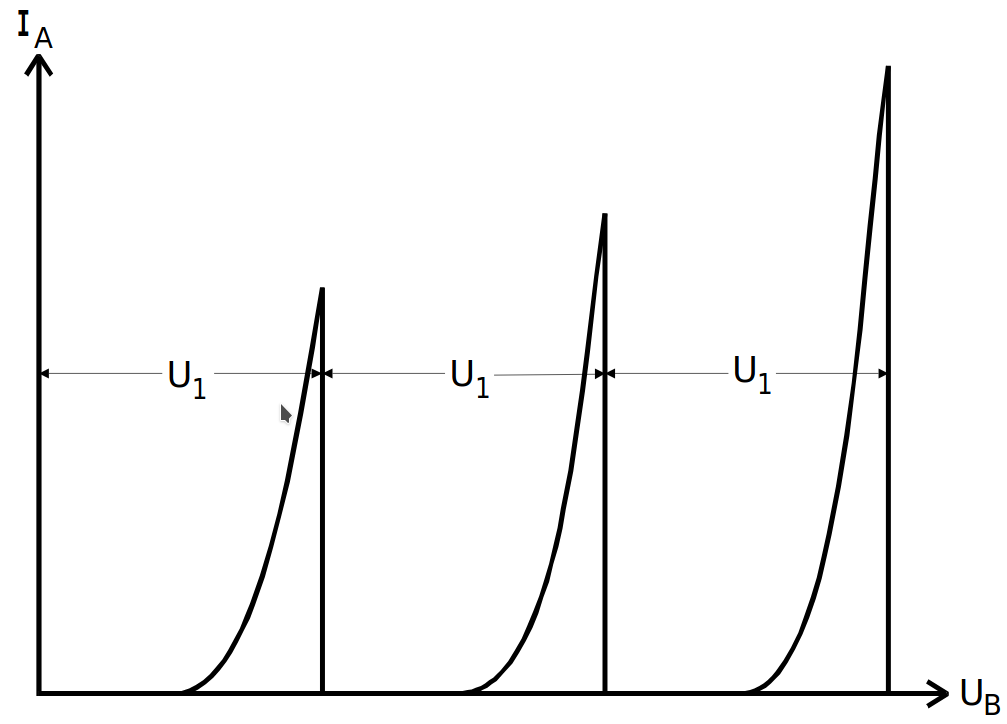
\includegraphics[width=0.75\textwidth]{content/data/Spannungsverlauf.png}
    \caption{Der schematische Spannungsverlauf der Franck-Hertz Kurven. Bild entnommen aus der Versuchsanleitung \cite[4]{anleitung}.}
    \label{fig:spannungsverlauf}
\end{figure}
Dieser Verlauf wird Franck-Hertz-Kurve genannt.
Es fällt auf, dass trotz immer größer werdener Spannung $U_\text{B}$, der Strom nach einem Maximum immer wieder auf 0 zurückfällt.
Das liegt daran, dass die Elektronen bei einer Energie von $U_\text{B} e = n(E_1 - E_0)$ all ihre Energie abgeben und deshalb die Auffängerelektrode nicht erreichen.
Das $n$ gibt dabei an wie viele mal die Energie der Elektronen der Anregungsenergie des Hg-Atoms entspricht.
Für eine vollständige Energieabgabe an das Atom muss $n$ also ganzzahlig sein.
\\\\
In der Realität sieht die Franck-Hertz-Kurve allerdings etwas abgerundeter aus, da nicht alle Elektronen die gleiche Energie aufweisen.
Zudem hat das Kontaktpotenial einen Einfluss auf die Kurve.
Da die Austrittsarbeit $\Phi_\text{G}$ des Glühdrahts wesentlich geringer ist als die der Beschleunigungselektrode $\Phi_\text{B}$ weisen sie ein Potentialgefälle auf.
Dieses ist graphisch in Abbildung \ref{fig:potential} verdeutlicht worden.
\begin{figure}
    \centering
    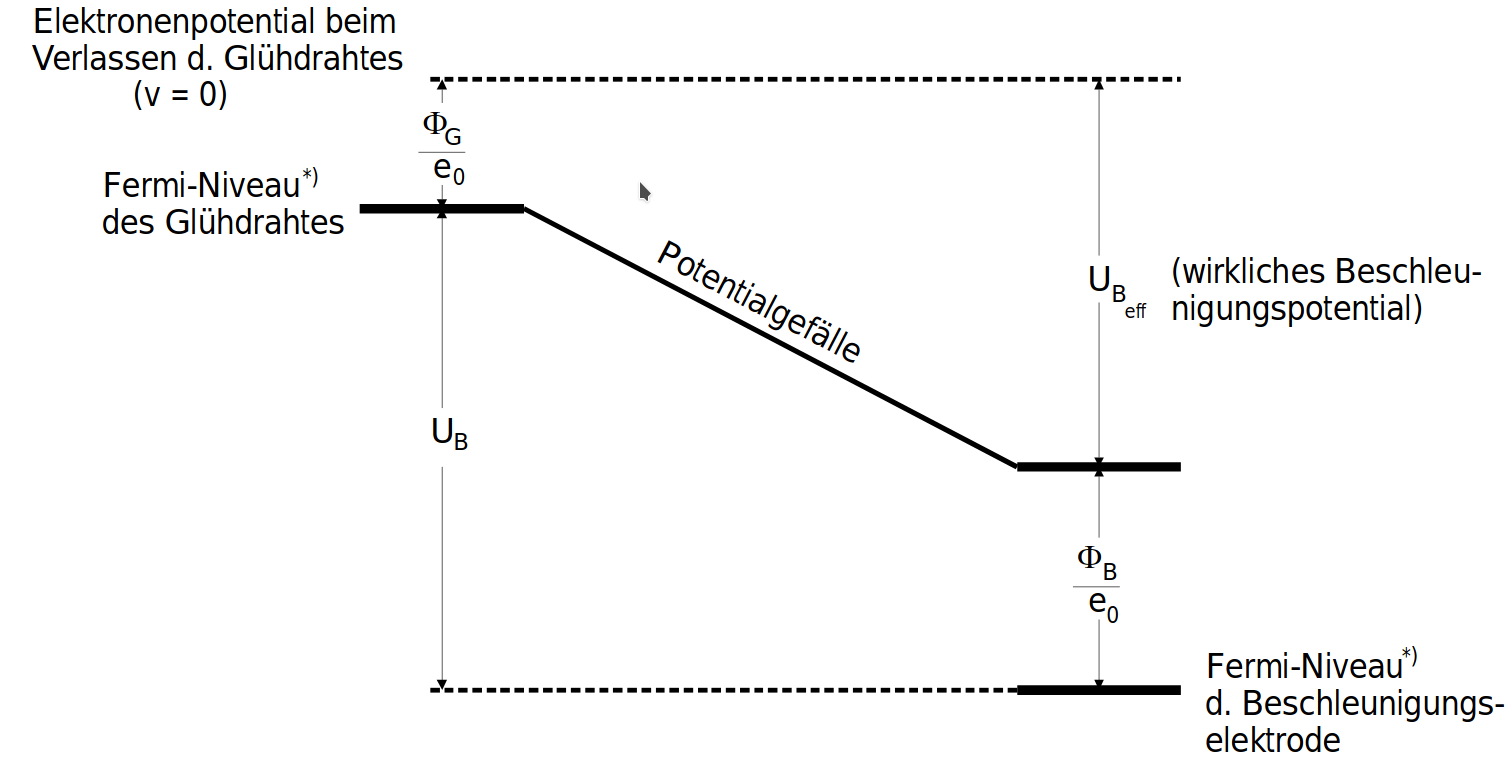
\includegraphics[width=\textwidth]{content/data/Potentialgefaelle.png}
    \caption{Das Potentiallgefälle zwischen Glühdraht und Beschleunigungselektrode. Bild entnommen aus der Versuchsanleitung \cite[5]{anleitung}.}
    \label{fig:potential}
\end{figure}
Das so entstehende Kontaktpotential $K$ lässt sich durch 
\begin{equation}
    K = \frac{1}{e} \left ( \Phi_\text{B} - \Phi_\text{G} \right)
    \label{eq:kontaktpotential}
\end{equation}
berechnen.
Damit hat das effektive Beschleunigungspotential $U_\text{B,eff}$ den Wert
\begin{equation}
    U_\text{B,eff} = U_\text{B} - K.
    \label{eq:beschleunigungeffektiv}
\end{equation}
\\\\
Zudem nimmt der Dampfdruck einen Einfluss auf die Kurve.
Denn umso höher der Dampfdruck ist, umso mehr Hg-Atome befinden sich in dem Rohr und die Wahrscheinlichkeit, dass ein Elektron ein Atom stößt nimmt zu.
Aus dem Dampfdruck lässt sich die mittlere freie Weglänge $\bar{w}$ zwischen den Hg-Atomen bestimmen.
Die entspricht der Formel
\begin{equation}
    \bar{w} = \frac{0.0029}{5.5\cdot10^7 \cdot \symup{e}^{-6876/T} },
\end{equation}
wobei $T$ der Temperatur entspricht.



